% !TeX program = xelatex
\documentclass[a4paper,12pt]{article}
% Личная преамбула и титульный лист; заполнить поля текущей работы.
\newcommand{\LabSubject}{Системы искусственного интеллекта}
\newcommand{\LabWorkType}{ЛАБОРАТОРНАЯ РАБОТА}
\newcommand{\LabNumber}{3}
\newcommand{\LabTopic}{Метод опорных векторов}
\newcommand{\LabVariant}{} % Пустое значение скрывает строку варианта.
\newcommand{\LabAuthor}{Михайлов Петр Сергеевич}
\newcommand{\LabGroup}{P3311}
\newcommand{\LabTeacher}{Королёва Юлия Александровна}
\newcommand{\LabYear}{\the\year}

\usepackage{iftex}
\ifPDFTeX
  \usepackage[T2A]{fontenc}
  \usepackage[utf8]{inputenc}
  \usepackage[russian]{babel}
\else
  \usepackage{fontspec}
  \usepackage{polyglossia}
  \setdefaultlanguage{russian}
  \setotherlanguage{english}
  \IfFontExistsTF{Times New Roman}{%
    \setmainfont{Times New Roman}\newfontfamily\cyrillicfont{Times New Roman}}{%
    \IfFontExistsTF{NimbusRoman-Regular.otf}{%
      \setmainfont{NimbusRoman}[Extension=.otf,UprightFont=*-Regular,BoldFont=*-Bold,ItalicFont=*-Italic,BoldItalicFont=*-BoldItalic]
      \newfontfamily\cyrillicfont{NimbusRoman}[Extension=.otf,UprightFont=*-Regular,BoldFont=*-Bold,ItalicFont=*-Italic,BoldItalicFont=*-BoldItalic]
    }{\setmainfont{DejaVu Serif}\newfontfamily\cyrillicfont{DejaVu Serif}}}
  \IfFontExistsTF{DejaVu Sans}{\setsansfont{DejaVu Sans}\newfontfamily\cyrillicfontsf{DejaVu Sans}}{%
    \IfFontExistsTF{NimbusSans-Regular.otf}{%
      \setsansfont{NimbusSans}[Extension=.otf,UprightFont=*-Regular,BoldFont=*-Bold,ItalicFont=*-Italic,BoldItalicFont=*-BoldItalic]
      \newfontfamily\cyrillicfontsf{NimbusSans}[Extension=.otf,UprightFont=*-Regular,BoldFont=*-Bold,ItalicFont=*-Italic,BoldItalicFont=*-BoldItalic]
    }{\setsansfont{Arial}\newfontfamily\cyrillicfontsf{Arial}}}
  \IfFontExistsTF{DejaVu Sans Mono}{\setmonofont{DejaVu Sans Mono}\newfontfamily\cyrillicfonttt{DejaVu Sans Mono}}{\setmonofont{Consolas}\newfontfamily\cyrillicfonttt{Consolas}}
\fi
\usepackage{amsmath,amssymb,amsfonts}
\usepackage{graphicx,geometry,listings,xcolor,hyperref,float,booktabs}
\usepackage{longtable,array,tabularx,caption}
\usepackage{tikz,pgfplots}
\usetikzlibrary{arrows.meta,fit,positioning}
\pgfplotsset{compat=1.18}
\geometry{left=2cm,right=1.5cm,top=2cm,bottom=2cm}
\hypersetup{unicode=true,colorlinks=true,linkcolor=black,citecolor=black,urlcolor=blue!60!black,
 pdftitle={\LabWorkType\space №\LabNumber. \LabTopic},pdfauthor={\LabAuthor}}
\captionsetup{font=small,labelsep=period}
\setlength{\parindent}{1.25cm}
\setlength{\parskip}{.2em}
\linespread{1.05}
\raggedbottom
\setcounter{tocdepth}{2}
\setlength{\emergencystretch}{2em}
\tolerance=3000
\lstdefinestyle{mypython}{language=Python,basicstyle=\ttfamily\scriptsize,
 keywordstyle=\color{blue!65!black}\bfseries,stringstyle=\color{red!65!black},
 commentstyle=\color{green!35!black},numbers=left,numberstyle=\tiny\color{gray},
 stepnumber=1,numbersep=7pt,showstringspaces=false,tabsize=4,frame=single,
 breaklines=true,breakatwhitespace=false,columns=fullflexible,keepspaces=true,
 xleftmargin=14pt,framexleftmargin=10pt,backgroundcolor=\color{gray!3}}
\lstset{style=mypython}

\begin{document}
\begin{titlepage}
\centering
{\fontsize{11}{13}\selectfont\textbf{Министерство науки и высшего образования Российской Федерации}}\\
{\fontsize{7}{10}\selectfont ФЕДЕРАЛЬНОЕ ГОСУДАРСТВЕННОЕ АВТОНОМНОЕ ОБРАЗОВАТЕЛЬНОЕ УЧРЕЖДЕНИЕ ВЫСШЕГО ОБРАЗОВАНИЯ}\\
\vspace{.2cm}
{\fontsize{14}{17}\selectfont\textbf{«НАЦИОНАЛЬНЫЙ ИССЛЕДОВАТЕЛЬСКИЙ УНИВЕРСИТЕТ ИТМО»}}
\vspace{1cm}

{\fontsize{12}{14}\selectfont\textbf{Факультет программной инженерии и компьютерной техники}}
\vspace{1cm}

{\fontsize{12}{14}\selectfont\textbf{Дисциплина: \LabSubject}}
\vspace*{\fill}

{\fontsize{18}{22}\selectfont\textbf{\LabWorkType\ №\LabNumber}}\\
\vspace{.5cm}
{\fontsize{14}{17}\selectfont\textbf{по теме: «\LabTopic»}}
\vspace{1.5cm}

\begin{flushright}
\fontsize{12}{14}\selectfont
Выполнил:\\
\LabAuthor\\
Группа: \LabGroup\\[1em]
Преподаватель:\\
\LabTeacher
\end{flushright}
\vfill
{\fontsize{12}{14}\selectfont Санкт-Петербург, \LabYear}
\end{titlepage}
\setcounter{page}{2}
{\small\setlength{\parskip}{0pt}\tableofcontents}
\newpage

\section{Цель и исходные данные}
Цель работы — реализовать линейный метод опорных векторов с мягким зазором, исследовать влияние регуляризации, размера мини-пакета и масштабирования, а также сравнить результат с собственной логистической регрессией.

Использован набор Banknote Authentication \cite{uci}: каждый объект описывает изображение банкноты четырьмя числовыми признаками \texttt{variance}, \texttt{skewness}, \texttt{curtosis}, \texttt{entropy}; целевая переменная \texttt{class} принимает значения 0 и 1. Первоначально набор содержит 1372 строки. Из них удалены 24 точные повторные записи без противоречий в метках, чтобы один и тот же объект не попал одновременно в обучающую и проверочную части. Осталось 1348 объектов.

Данные случайно и стратифицированно делятся на обучающую, валидационную и тестовую выборки с фиксированным начальным состоянием генератора 6752. Для стандартизации среднее $\mu_j$ и стандартное отклонение $\sigma_j$ каждого признака вычисляются только по обучающей части; затем все три части преобразуются по формуле $z_j=(x_j-\mu_j)/\sigma_j$. Настройки выбираются на validation, а test используется для итоговой оценки. Для сравнения без масштабирования применяется то же разбиение.

\section{Метод}
Модель вычисляет оценку $s(\mathbf{x})=\mathbf{w}^{T}\mathbf{x}+b$, а метки классов внутри SVM записываются как $y\in\{-1,+1\}$. Знак оценки задаёт предсказанный класс. Функциональный отступ объекта равен $m_i=y_i s(\mathbf{x}_i)$. Линии $s=\pm1$ ограничивают полосу шириной $2/\lVert\mathbf w\rVert$.

Оптимизируемая функция для $N$ обучающих объектов имеет вид
\begin{equation}\label{eq:objective}
J(\mathbf w,b)=\frac{\lambda}{2}\lVert\mathbf w\rVert^2+\frac1N\sum_{i=1}^{N}\max\bigl(0,1-y_i(\mathbf w^T\mathbf x_i+b)\bigr).
\end{equation}
Здесь первое слагаемое — L2-регуляризация весов, второе — средняя hinge loss. Свободный член $b$ не штрафуется. Чем больше $\lambda$, тем сильнее ограничиваются веса. Правильно классифицированный объект всё ещё может давать ненулевые потери при $0<m_i<1$.

Для пакета $B$ объекты с $m_i<1$ дают вклад в субградиент hinge loss:
\begin{equation}\label{eq:gradient}
g_w=\lambda\mathbf w-\frac{1}{|B|}\sum_{i\in B:m_i<1}y_i\mathbf x_i,\qquad
g_b=-\frac{1}{|B|}\sum_{i\in B:m_i<1}y_i.
\end{equation}
В точке $m_i=1$ выбирается допустимый нулевой вклад hinge loss. После каждого пакета веса и свободный член обновляются с постоянным шагом; перед каждой эпохой порядок объектов перемешивается. В истории сохраняются средняя hinge loss и полная функция \eqref{eq:objective}.

Положительным считается класс 1. Accuracy, precision, recall и F1 рассчитываются через элементы матрицы ошибок. ROC-кривая показывает зависимость полноты от доли ложноположительных ответов, PR-кривая — точности от полноты. Площади ROC-AUC и PR-AUC вычисляются методом трапеций по непрерывным оценкам; в начальной точке PR-кривой при отсутствии положительных предсказаний принято precision $=1$. Одинаковые значения score обрабатываются одновременно. Для SVM используется \texttt{decision\_function}, для логистической регрессии — \texttt{predict\_proba}.

\section{План эксперимента и выбор настроек}
Стратифицированное разбиение содержит 808 объектов train, 269 validation и 271 test. Для SVM рассмотрены $\lambda\in\{0{,}001;\,0{,}01;\,0{,}1;\,1\}$ и размеры пакета 32, 128 и 808. Шаг обучения равен 0,01; каждое сочетание проверялось со стандартизацией и без неё до 1200 эпох. Выбор делался по минимальной validation hinge loss, то есть без добавления штрафа к критерию оценки на validation. Минимум определялся внутри истории каждого запуска, затем сравнивались полученные конфигурации.

\begin{figure}[H]\centering
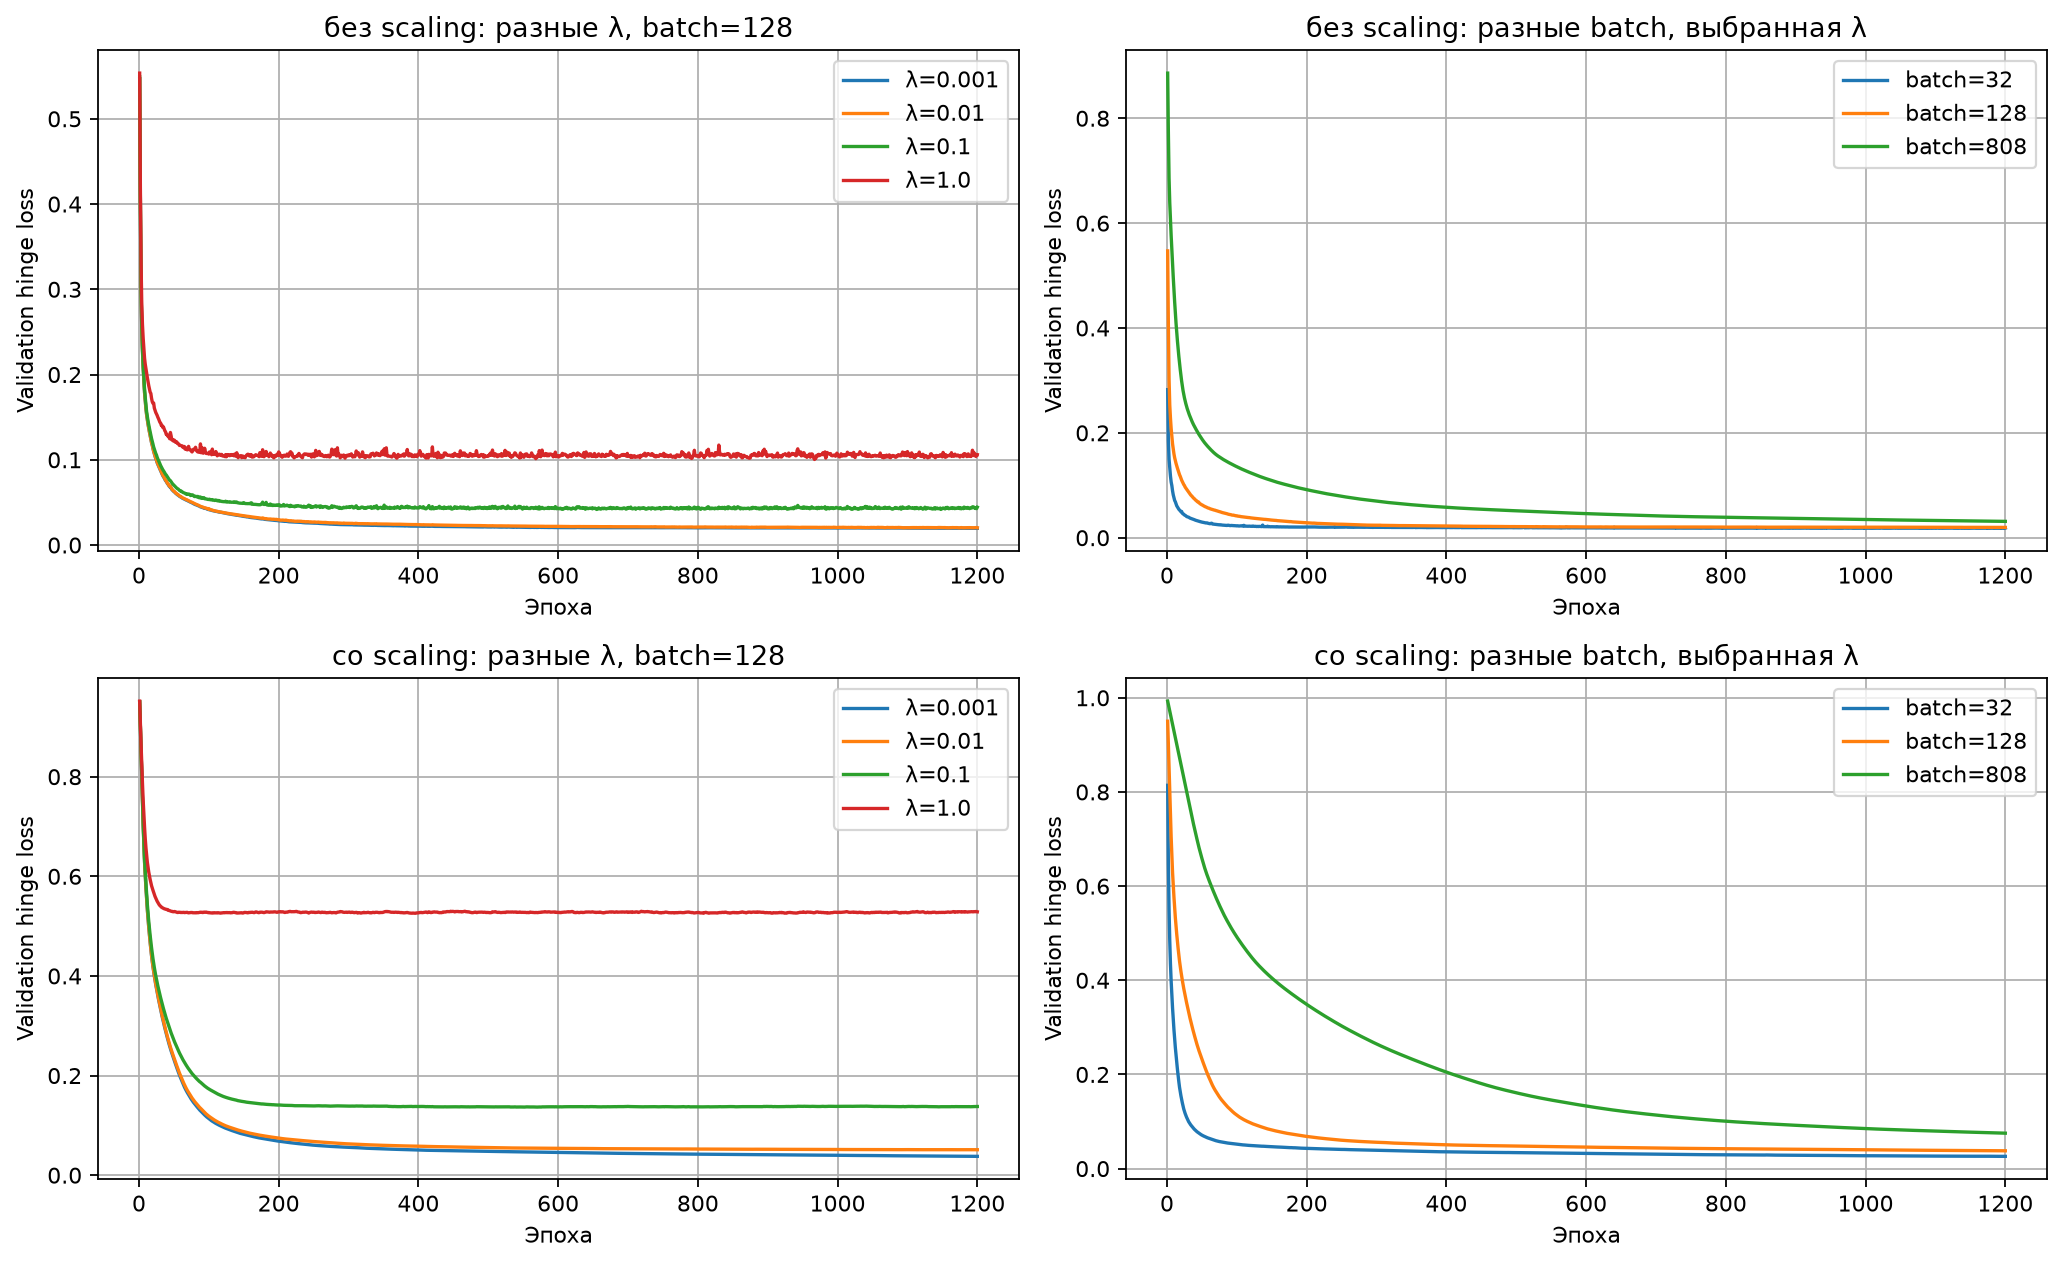
\includegraphics[width=\textwidth]{figures/validation_epochs.png}
\caption{Validation hinge loss в нескольких запусках с разной регуляризацией и размерами пакетов.}\label{fig:epochs}
\end{figure}
\begin{figure}[H]\centering
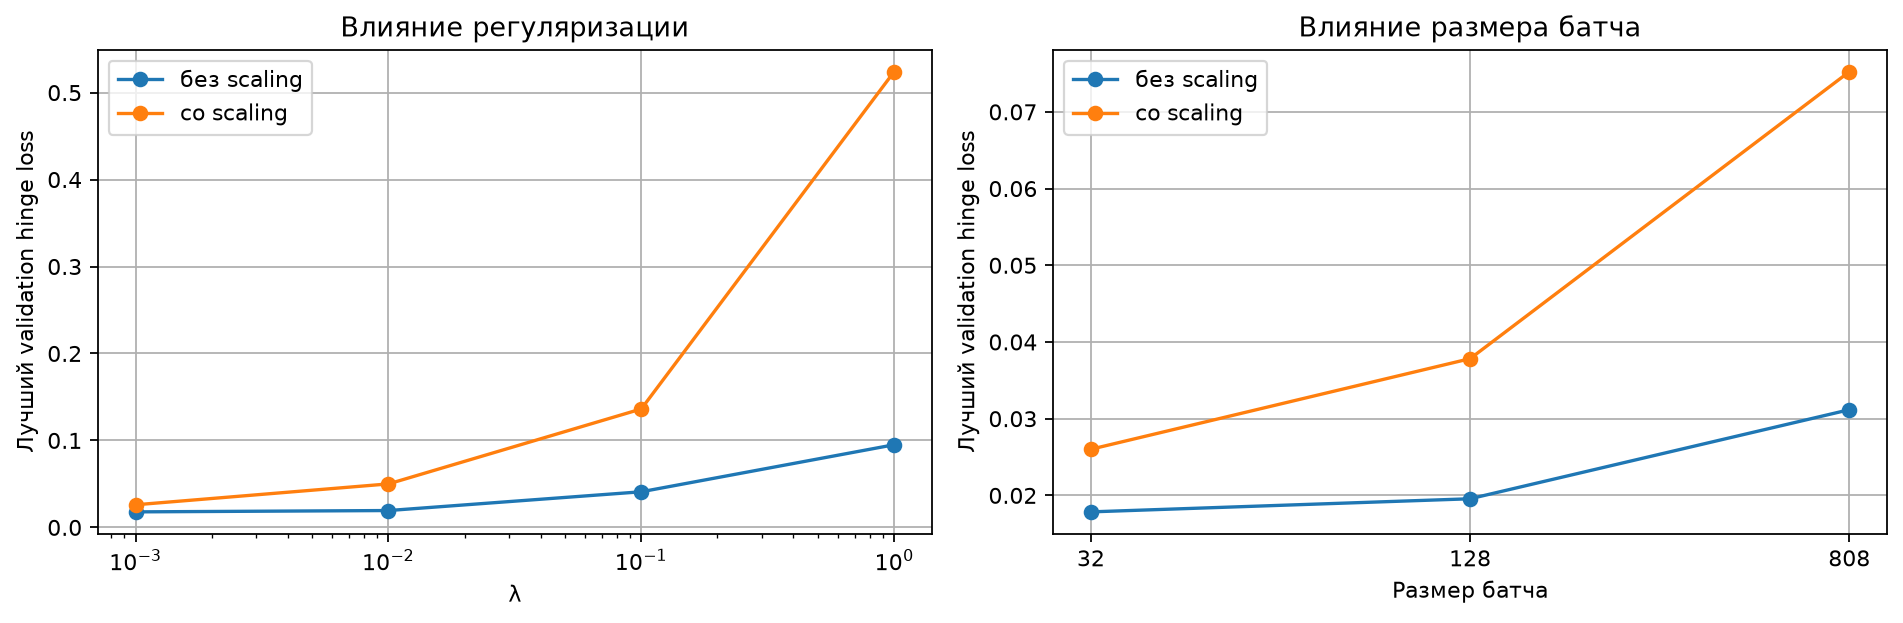
\includegraphics[width=\textwidth]{figures/hyperparameters.png}
\caption{Лучшие значения validation hinge loss при изменении $\lambda$ и размера пакета.}\label{fig:search}
\end{figure}

По validation выбрана модель без масштабирования: $\lambda=0{,}001$, пакет из 32 объектов и 1198 эпох, validation hinge loss $0{,}01785$. Лучший масштабированный вариант использует те же $\lambda$ и размер пакета, 1199 эпох и достигает $0{,}02601$. При этом исходные и стандартизованные признаки задают разную геометрию штрафа; сравнение относится к указанной сетке и одному разбиению, а не доказывает, что масштабирование всегда ухудшает SVM. Графики на рис.~\ref{fig:epochs} и \ref{fig:search} показывают динамику разных запусков и результаты поиска. При большем пакете за эпоху выполняется меньше обновлений, поэтому сравнение при равном числе эпох не означает равного числа шагов.

Число 1198 — минимум среди проверенных эпох выбранного запуска. Он расположен рядом с границей 1200, а validation loss ещё медленно уменьшается; данных недостаточно, чтобы объявить это число глобальным оптимумом или исключить улучшение при более длинном обучении. В предварительном диапазоне до 600 эпох минимум составлял $0{,}01861$, поэтому бюджет был расширен. Изменение до $0{,}01785$ показывает улучшение, хотя оно невелико. Истории потерь выбранной конфигурации приведены на рис.~\ref{fig:training}.

\begin{figure}[H]\centering
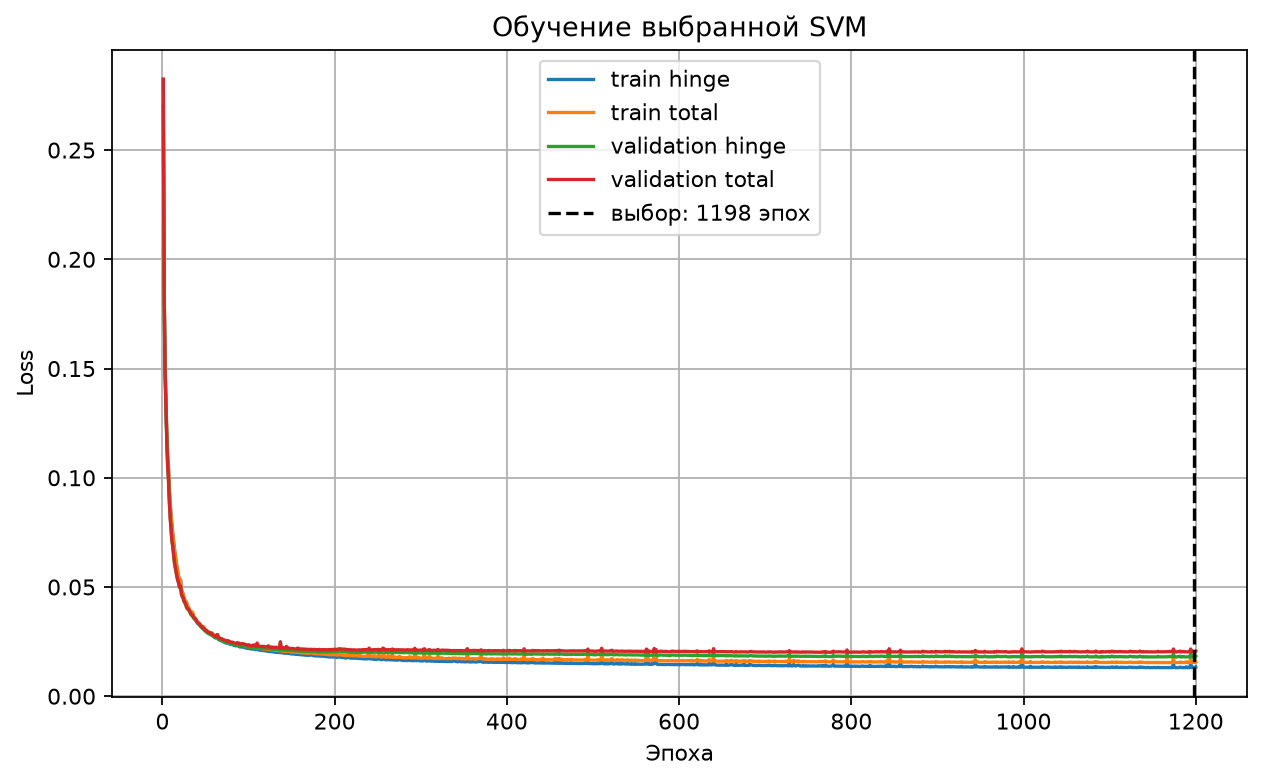
\includegraphics[width=.85\textwidth]{figures/learning_curves.png}
\caption{Hinge и полная функция потерь для train и validation выбранной SVM.}\label{fig:training}
\end{figure}

Логистическая регрессия из ЛР1 обучалась на тех же объектах с train-стандартизацией. Проверены шаги 0,05, 0,5 и 1,0 и бюджеты 250, 1000, 3000, 6000 и 12000 эпох. Минимальная validation BCE, $0{,}01448$, получена при шаге 1,0 и 12000 эпохах. Этот минимум тоже находится на границе проверенного диапазона, поэтому 12000 — выбранный проверенный бюджет, а не доказанная оптимальная длительность. Кривые нескольких запусков и validation BCE показаны на рис.~\ref{fig:logistic}.
\begin{figure}[H]\centering
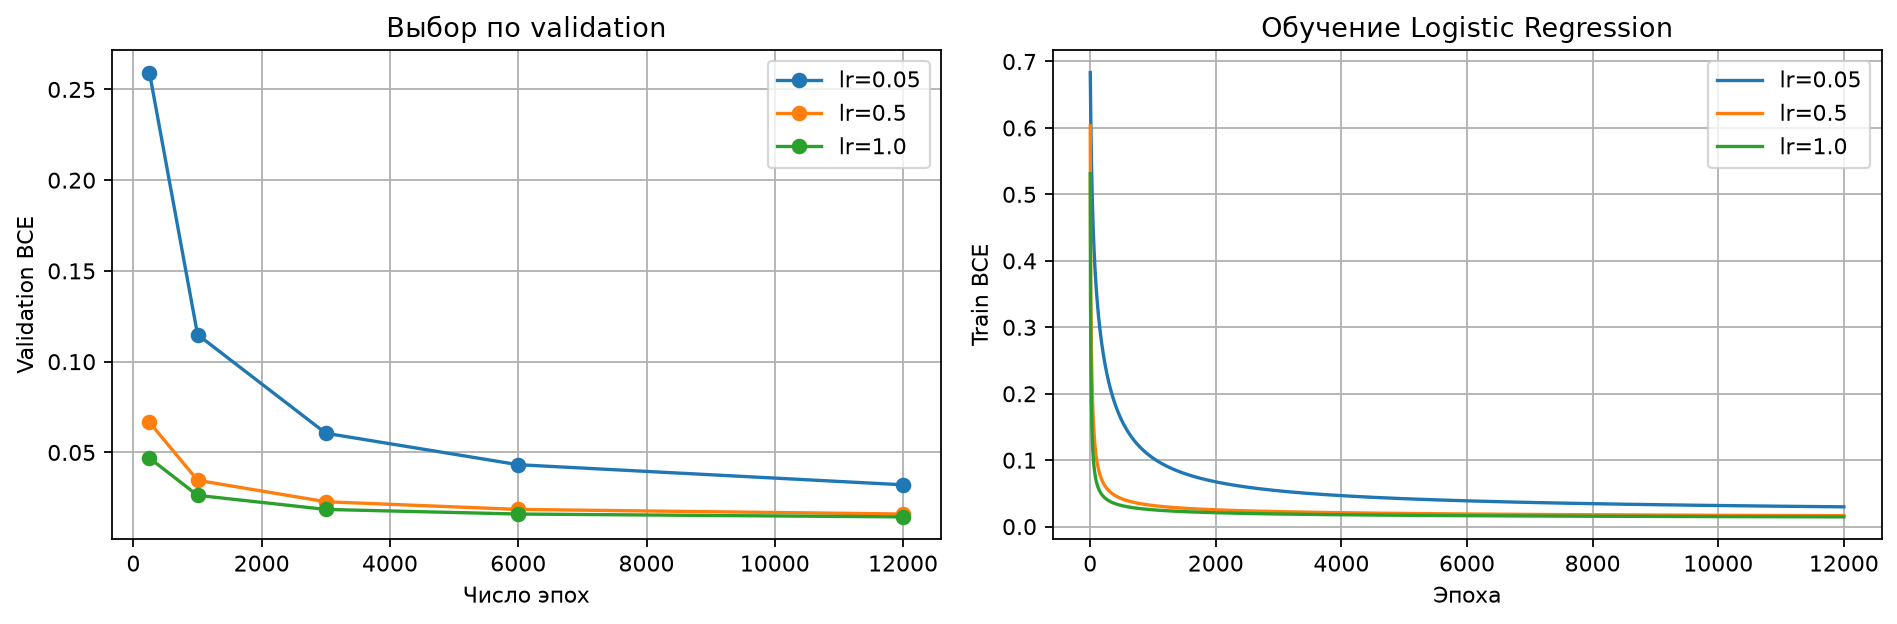
\includegraphics[width=\textwidth]{figures/logistic_learning.png}
\caption{Обучение логистической регрессии и сравнение validation BCE по бюджетам.}\label{fig:logistic}
\end{figure}

\section{Результаты на тестовой выборке}
Все настройки и способ масштабирования были определены до расчёта на test. Для полноты отдельно показан и заранее выбранный лучший вариант SVM со стандартизацией. В таблице~\ref{tab:metrics} приведены значения для положительного класса 1.
\begin{table}[H]\centering\small
\caption{Метрики на test}\label{tab:metrics}
\begin{tabular}{lrrrrrr}\toprule
Модель & Accuracy & Precision & Recall & F1 & ROC-AUC & PR-AUC \\\midrule
SVM без scaling & 0,9963 & 1,0000 & 0,9918 & 0,9959 & 1,0000 & 1,0000 \\
SVM со scaling & 0,9926 & 0,9918 & 0,9918 & 0,9918 & 0,9999 & 0,9999 \\
Логистическая регрессия & 0,9963 & 1,0000 & 0,9918 & 0,9959 & 0,9999 & 0,9999 \\\bottomrule
\end{tabular}
\end{table}

Выбранная SVM на test допустила одну ложноотрицательную ошибку и не допустила ложноположительных: матрица ошибок показана на рис.~\ref{fig:matrix}. При фиксированных порогах SVM и логистическая регрессия дали одинаковые значения четырёх классификационных метрик; их ранжирование немного отличается. Равные единице ROC-AUC и PR-AUC SVM означают идеальное ранжирование именно на этой конечной test-выборке, но не гарантируют безошибочность при пороге ноль и на новых данных. ROC и PR-кривые показаны на рис.~\ref{fig:rocpr}, сравнение метрик — на рис.~\ref{fig:comparison}.

\begin{figure}[H]\centering
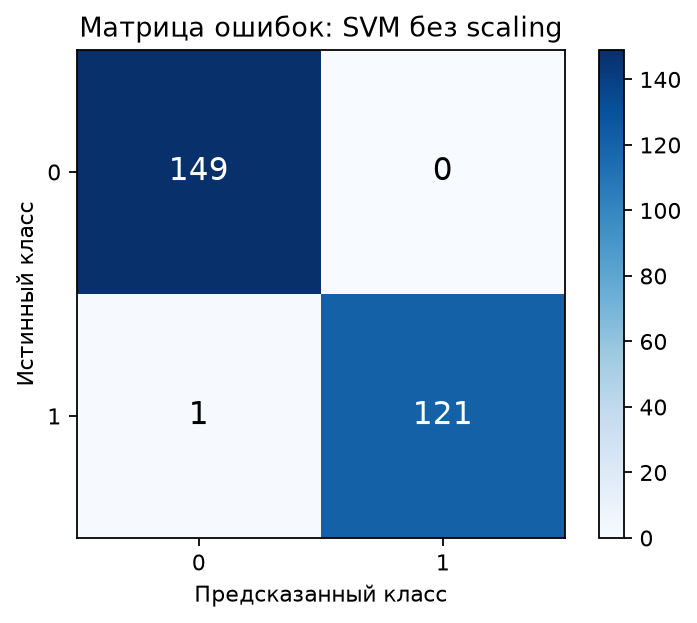
\includegraphics[width=.57\textwidth]{figures/confusion_matrix.png}
\caption{Матрица ошибок выбранной SVM на test.}\label{fig:matrix}
\end{figure}
\begin{figure}[H]\centering
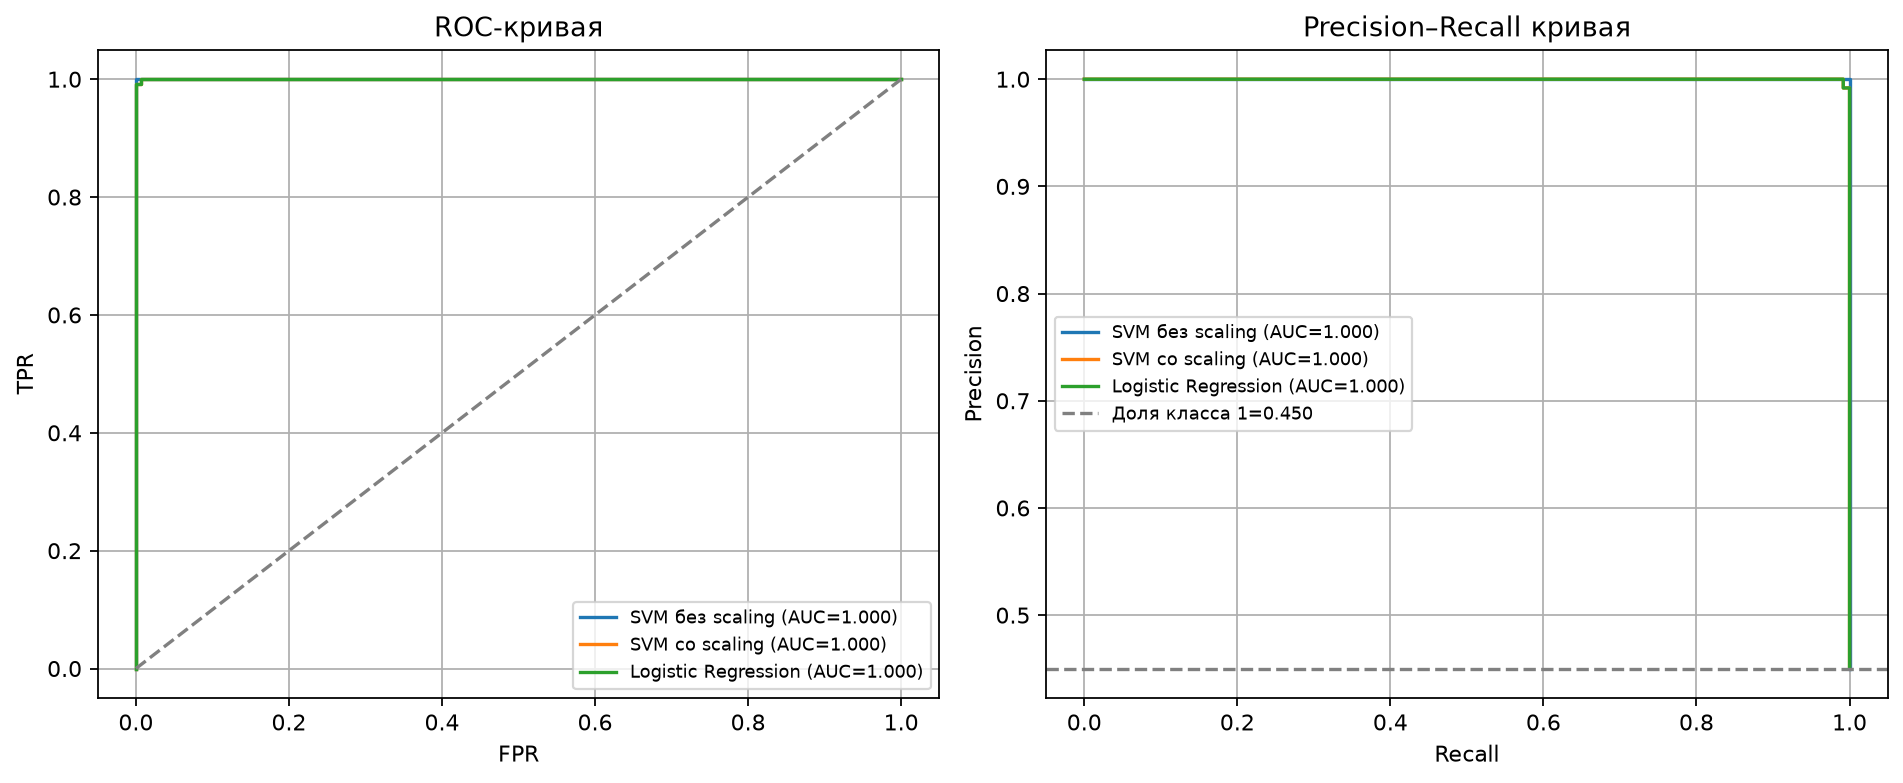
\includegraphics[width=\textwidth]{figures/roc_pr.png}
\caption{ROC и Precision–Recall кривые на test.}\label{fig:rocpr}
\end{figure}
\begin{figure}[H]\centering
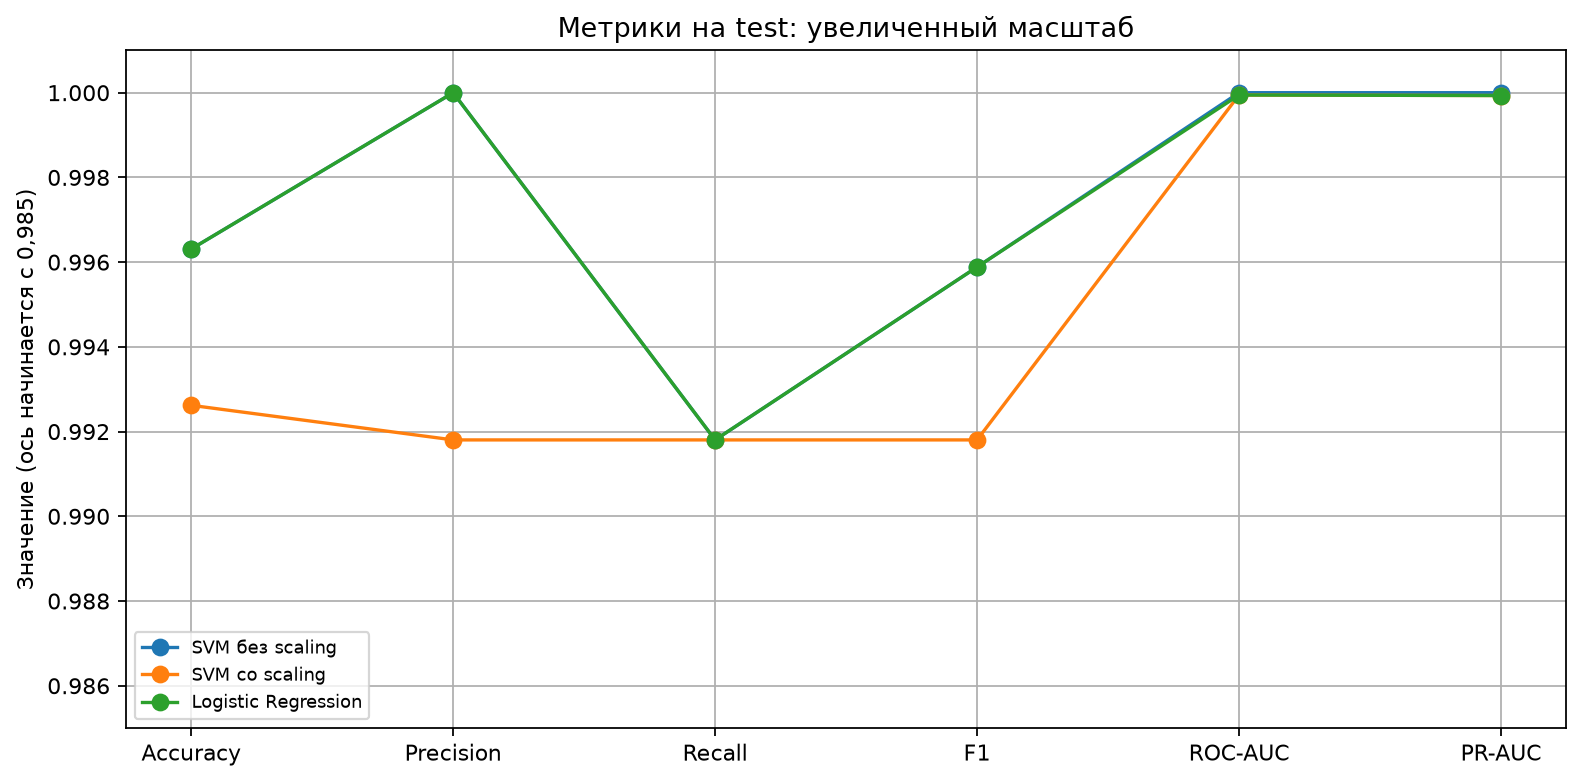
\includegraphics[width=.95\textwidth]{figures/model_comparison.png}
\caption{Сравнение классификационных и ранговых метрик на test.}\label{fig:comparison}
\end{figure}

\section{Двумерная визуализация}
Отдельная SVM обучена на признаках \texttt{variance} и \texttt{skewness}. На рис.~\ref{fig:2d} сплошная линия соответствует $s=0$, пунктирные — $s=\pm1$; обведены обучающие объекты с $y_i s_i\leq1$. Таких объектов 209 из 808. В их число входят как лежащие внутри полосы, так и неправильно классифицированные за её пределами. Это визуализация геометрии другой, двумерной модели; значения таблицы~\ref{tab:metrics} получены на всех четырёх признаках.
\begin{figure}[H]\centering
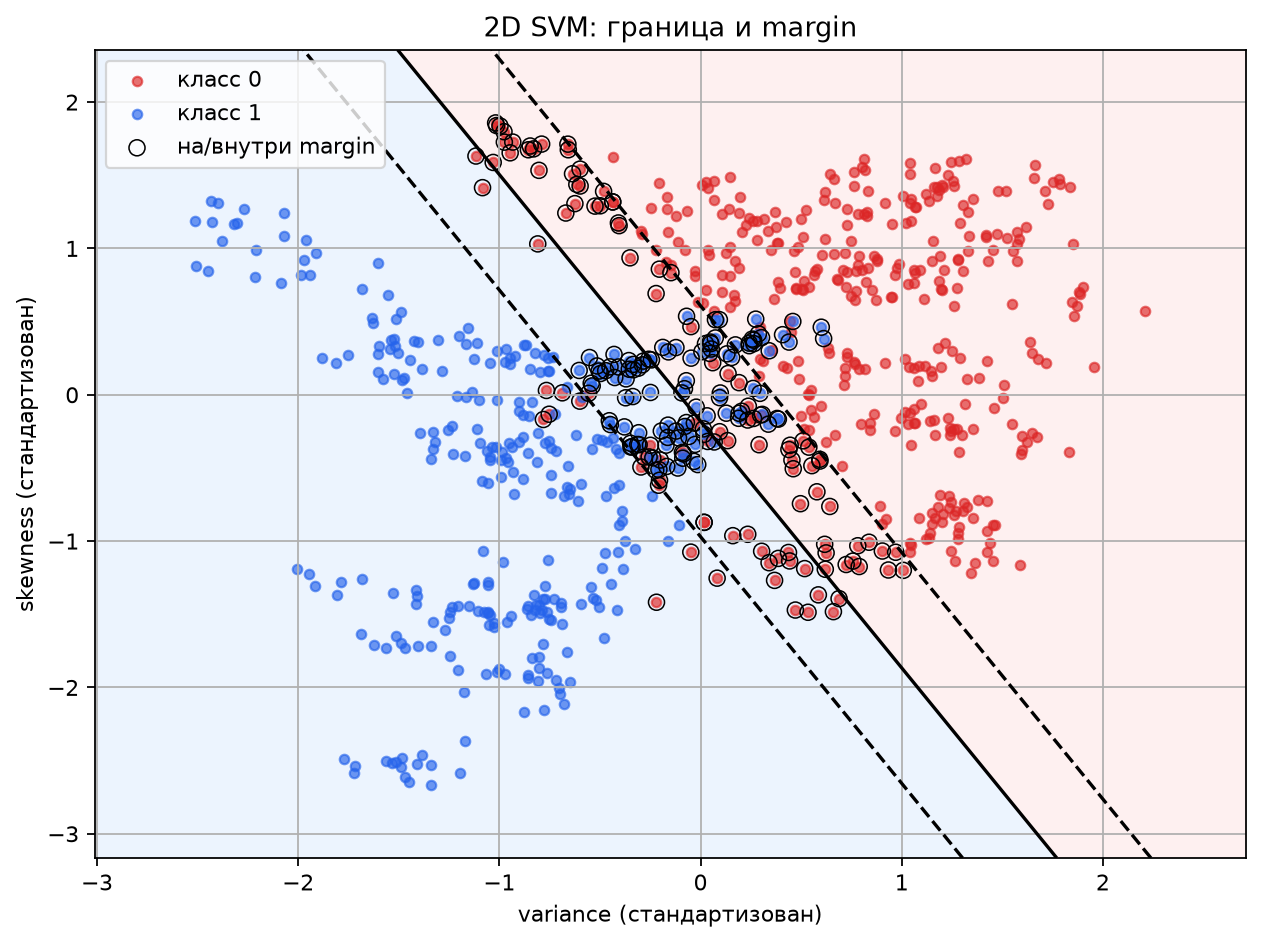
\includegraphics[width=.82\textwidth]{figures/svm_2d.png}
\caption{Разделяющая граница и линии margin двумерной SVM.}\label{fig:2d}
\end{figure}

\section{Вывод}
На рассмотренной сетке лучшая validation hinge loss получена без scaling при $\lambda=0{,}001$ и размере пакета 32; выбранная эпоха — 1198 из проверенных 1200. Для этого набора и сетки стандартизация не улучшила validation hinge loss. Сильная регуляризация на графиках приводит к более высокой потере и указывает на недообучение; выраженного расхождения train и validation у выбранной модели не видно, однако одно разбиение не исключает переобучения на validation при многократном подборе. Результаты test для SVM и логистической регрессии близки. ROC-AUC и PR-AUC оценивают ранжирование по непрерывному score; в отличие от них метрики матрицы ошибок относятся к одному порогу.

Исходный код и ноутбук доступны в \href{https://github.com/Axe-On-You/Artificial-intelligence-systems/tree/main/\%D0\%9B\%D0\%B0\%D0\%B1\%D0\%BE\%D1\%80\%D0\%B0\%D1\%82\%D0\%BE\%D1\%80\%D0\%BD\%D0\%B0\%D1\%8F\%203}{папке лабораторной работы в репозитории}.

\begin{thebibliography}{9}
\bibitem{uci} Lohweg V. Banknote Authentication. UCI Machine Learning Repository, 2012. DOI: \href{https://doi.org/10.24432/C55P57}{10.24432/C55P57}.
\end{thebibliography}
\end{document}
